\begin{figure}
  \centering
  \begin{subfigure}[b]{0.48\textwidth}
    \begin{tikzpicture}
      \node[inner sep=0pt] (img1) at (0.0, 0.0)
           {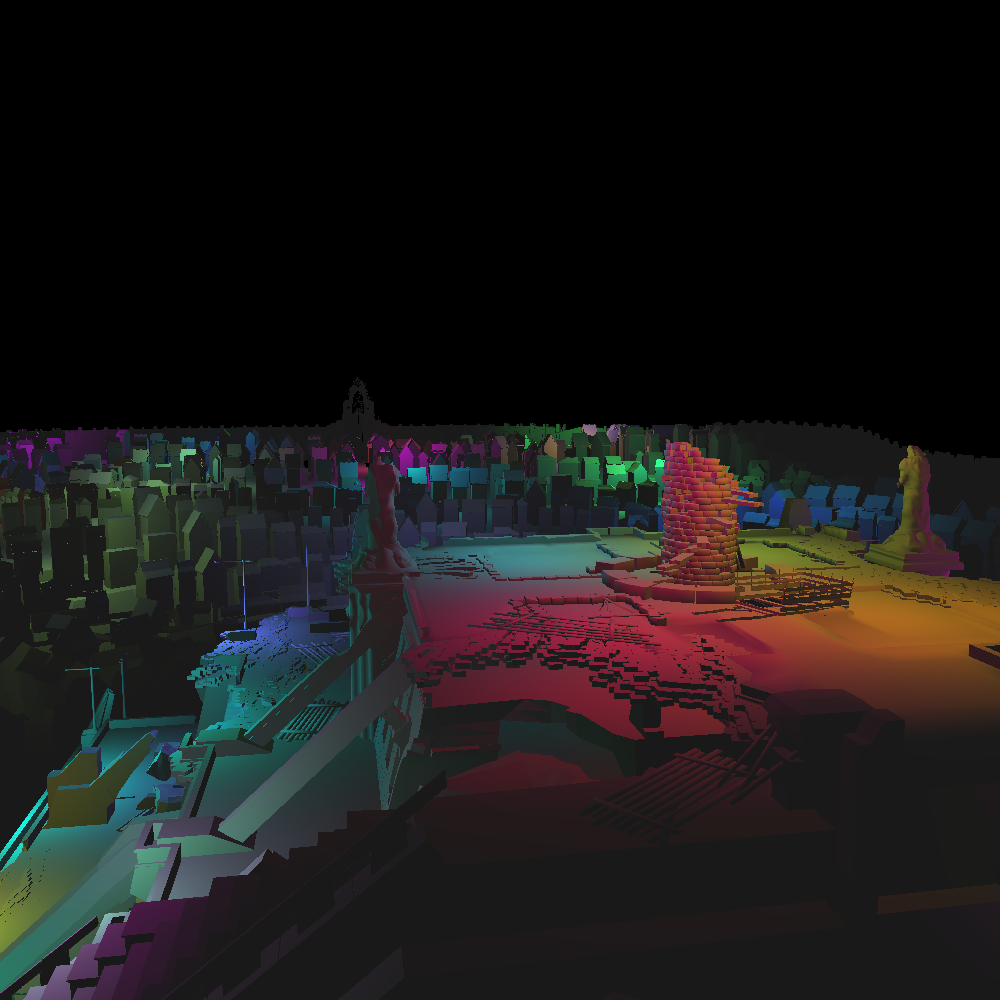
\includegraphics[width=\textwidth]{./img/raw/ts-grid-intro/frame_frame_400.png}};

      \foreach \i in {1, ..., 15} {
        \node at (-0.5\textwidth, -0.5\textwidth + 0.0625\textwidth * \i) (y_low) [] {};
        \node at (0.5\textwidth, -0.5\textwidth + 0.0625\textwidth * \i) (y_high) [] {};
        \draw[white, line width=0.025mm] (y_low.center) -- (y_high.center);
      }

      \foreach \i in {1, ..., 15} {
        \node at (-0.5\textwidth + 0.0625\textwidth * \i, -0.5\textwidth) (y_low) [] {};
        \node at (-0.5\textwidth + 0.0625\textwidth * \i, 0.5\textwidth) (y_high) [] {};
        \draw[white, line width=0.025mm] (y_low.center) -- (y_high.center);
      }
    \end{tikzpicture}
    \caption{Opdeling van een frame met resolutie $1024 \times 1024$ met tegels van $64 \times 64$ pixels.}
    \label{fig:ts-grid-intro:frame}
  \end{subfigure}\quad
  \begin{subfigure}[b]{0.48\textwidth}
    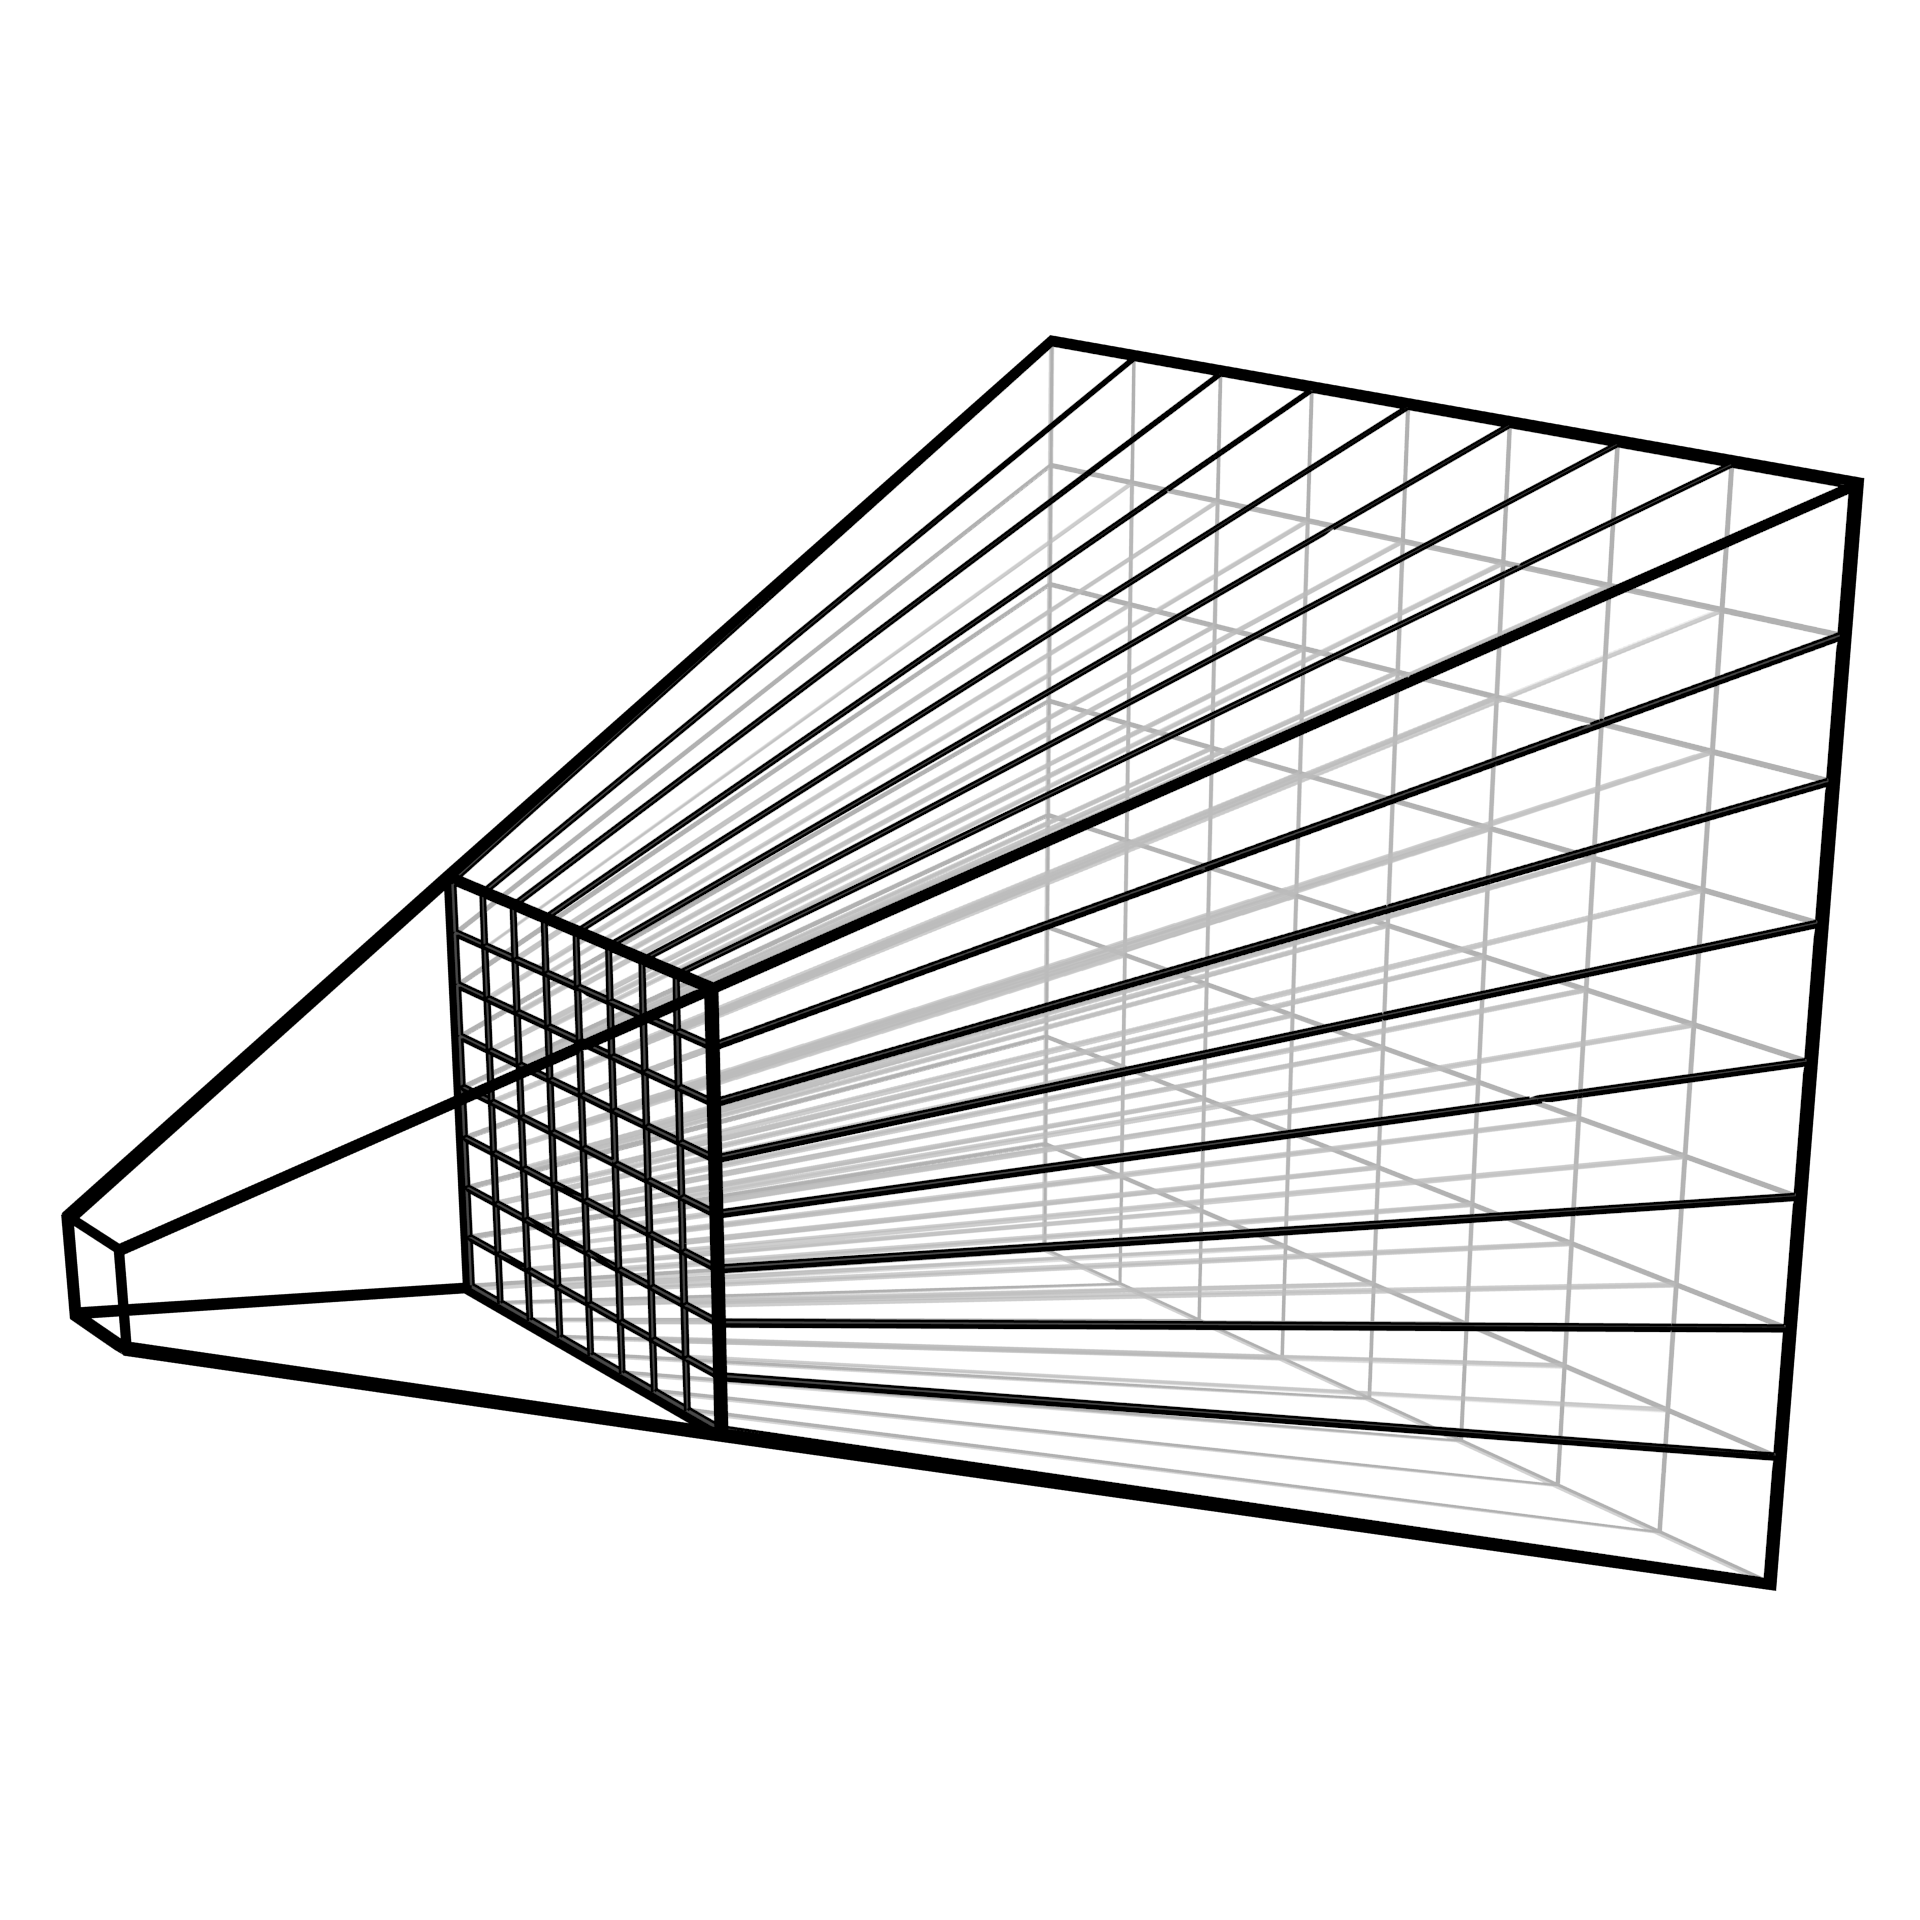
\includegraphics[width=\textwidth]{./img/raw/ts-grid-intro/frustum-opdeling.png}
    \caption{Opdeling van het zichtfrustum.}
    \label{fig:ts-grid-intro:frustum}
  \end{subfigure}
  \caption{Opdeling van het zichtveld.}
  \label{fig:ts-grid-intro}
\end{figure}

